\documentclass[10pt,norsk,a4paper]{article}
\usepackage[utf8]{inputenc}
\usepackage[T1]{fontenc}
\usepackage[norsk]{babel}
\usepackage[cm]{fullpage}
\usepackage{color}
\usepackage{parskip,textcomp,amssymb,graphicx}
\usepackage{pdfpages}
\usepackage[stable]{footmisc}
\usepackage{multicol}


\title{Generalforsamling \\
	Høst 2018\\[3cm]
	
\includegraphics[width=3cm,trim=0 4cm 0 0]{../../res/logo.png}\\}
\date{21.\ november 2018}
\author{Ifi-dagen}

% Blank header, samt footer med side x av y
\usepackage{fancyhdr}
\pagestyle{fancy}
\renewcommand{\headrulewidth}{0pt}
\fancyhead{}
\cfoot{Side~\thepage\ av~\pageref{lastpage}}


\begin{document}

\maketitle{}
\newpage
\part{Dagsorden og detaljer}
\tableofcontents{}
\newpage


\section{Valg av møteleder}

\section{Valg av referent}

\section{Valg av protokollunderskrivere}

\section{Valg av tellekorps}

\section{Godkjenning av innkalling}

\section{Godkjenning av dagsorden}

\section{Årsberetning v/ leder}
Hei Ifi-studenter og foreningsaktive!

\begin{multicols}{2}
Året 2018 har vært et spennende og utfordrende år. Det har vært en enorm
økning i interessen for karrieredager fra bedriftenes side, som førte til at
vi økte kapasiteten fra 41 til 54 bedrifter, hvorav 4 startups. DNB meldte
interesse for å bli hovedsamarbeidspartner tidlig på vårsemesteret, som var en
smått overraskende, men også positiv endring fra å utelukkende ha
konsulentselskaper. Interesseøkningen har også ført til et markant større
resultat enn tidligere, som er noe Ifi-foreninger forhåpentligvis vil nyte
godt av i lang tid framover.

Vi holdt i år tre store arrangementer: ettermiddagen@ifi, master-kickoff og 
dagen@ifi. Ettermiddagen@ifi ble gjennomført uten store forandringer fra
tidligere, med unntak av en økning i antall deltakende bedrifter fra 10 til 17.
Med bidrag fra et par sentrale interne gikk alt godt for seg, med en noe
forsinket matservering og standup som ikke traff klientellet helt.
Master-kickoff ble gjennomført hovedsakelig i regi av DNB, med matservering,
samtlige foredrag og en interaktiv hacke-konkurranse.

Under dagen@ifi, hadde vi -- grunnet økningen i antall deltakende bedrifter --
et større standområde en tidligere, som strakk seg helt til enden av gangen.
På dagtid hadde vi mange lærerike foredrag, et standområde som så og si til en
hver tid var fylt og flere runder med matservering. Så og si alt gikk ganske
smertefritt og alle de deltakende fikk seg til og med en obligatorisk
luftepause da brannalarmen ble utløst. På kveldstid gikk det meste knirkefritt,
med unntak av litt forsinkelser i opprigg av lounge-området og barer. Alt i alt
gikk arrangementet veldig bra.

Til tross for godt gjennomførte arrangementer, kan det ikke sies å ha vært
uten utfordringer. Med økningen i antall deltakende bedrifter, har det også
blitt stilt større krav til styret. Ansvarsfordelingen ble forsøkt løst med et
større fokus på å utforme en intern base med tanke på arbeidsgrupper, hvor vi
endte opp med noen sentrale bidragsytere. Dette var dessverre ikke nok med
tanke på arbeidsmengden, og finnes det et område Ifi-dagen burde fokusere på
framover, er det å bygge opp en internbase, samt en følelse av tilhørighet til
foreningen.

Selv om året som har gått har vært utfordrende, har det også vært en utrolig
positiv og lærerik opplevelse. Med et styre som jobbet iherdig i ukene opp mot
arrangementene, interne som støttet opp og alle funksjonærene som jobbet før,
under og etter dagen@ifi, har vi fått til å gjennomføre det største året for
Ifi-dagen som forening noen sinne. Det har vært en veldig positiv erfaring som
jeg lenge vil dra nytte av.
\end{multicols}

Takk.

Mvh. \\
Karl Hole Totland \\
Avtroppende leder \\

\section{Regnskap og revidert budsjett}
Økonomiansvarlig orienterer.

\subsection{Regnskap for 2018}
Økonomiansvarlig legger fram regnskapsresultatet for 2018.

\subsection{Budsjett for 2019}
Økonomiansvarlig legger fram tentativt forslag til budsjett for 2019.

\section{Valg}

\subsection{Leder}
\subsection{Nestleder}
\subsection{Økonomiansvarlig}
\subsection{Bedriftsansvarlig}
\subsection{Faglig ansvarlig}
\subsection{Funksjonæransvarlig}
\subsection{Promoteringsansvarlig}
\subsection{Teknisk ansvarlig}
\subsection{Underholdningsansvarlig}
\subsection{Sosialansvarlig}\label{lastpage}

\newpage
\part{Nåværende vedtekter}
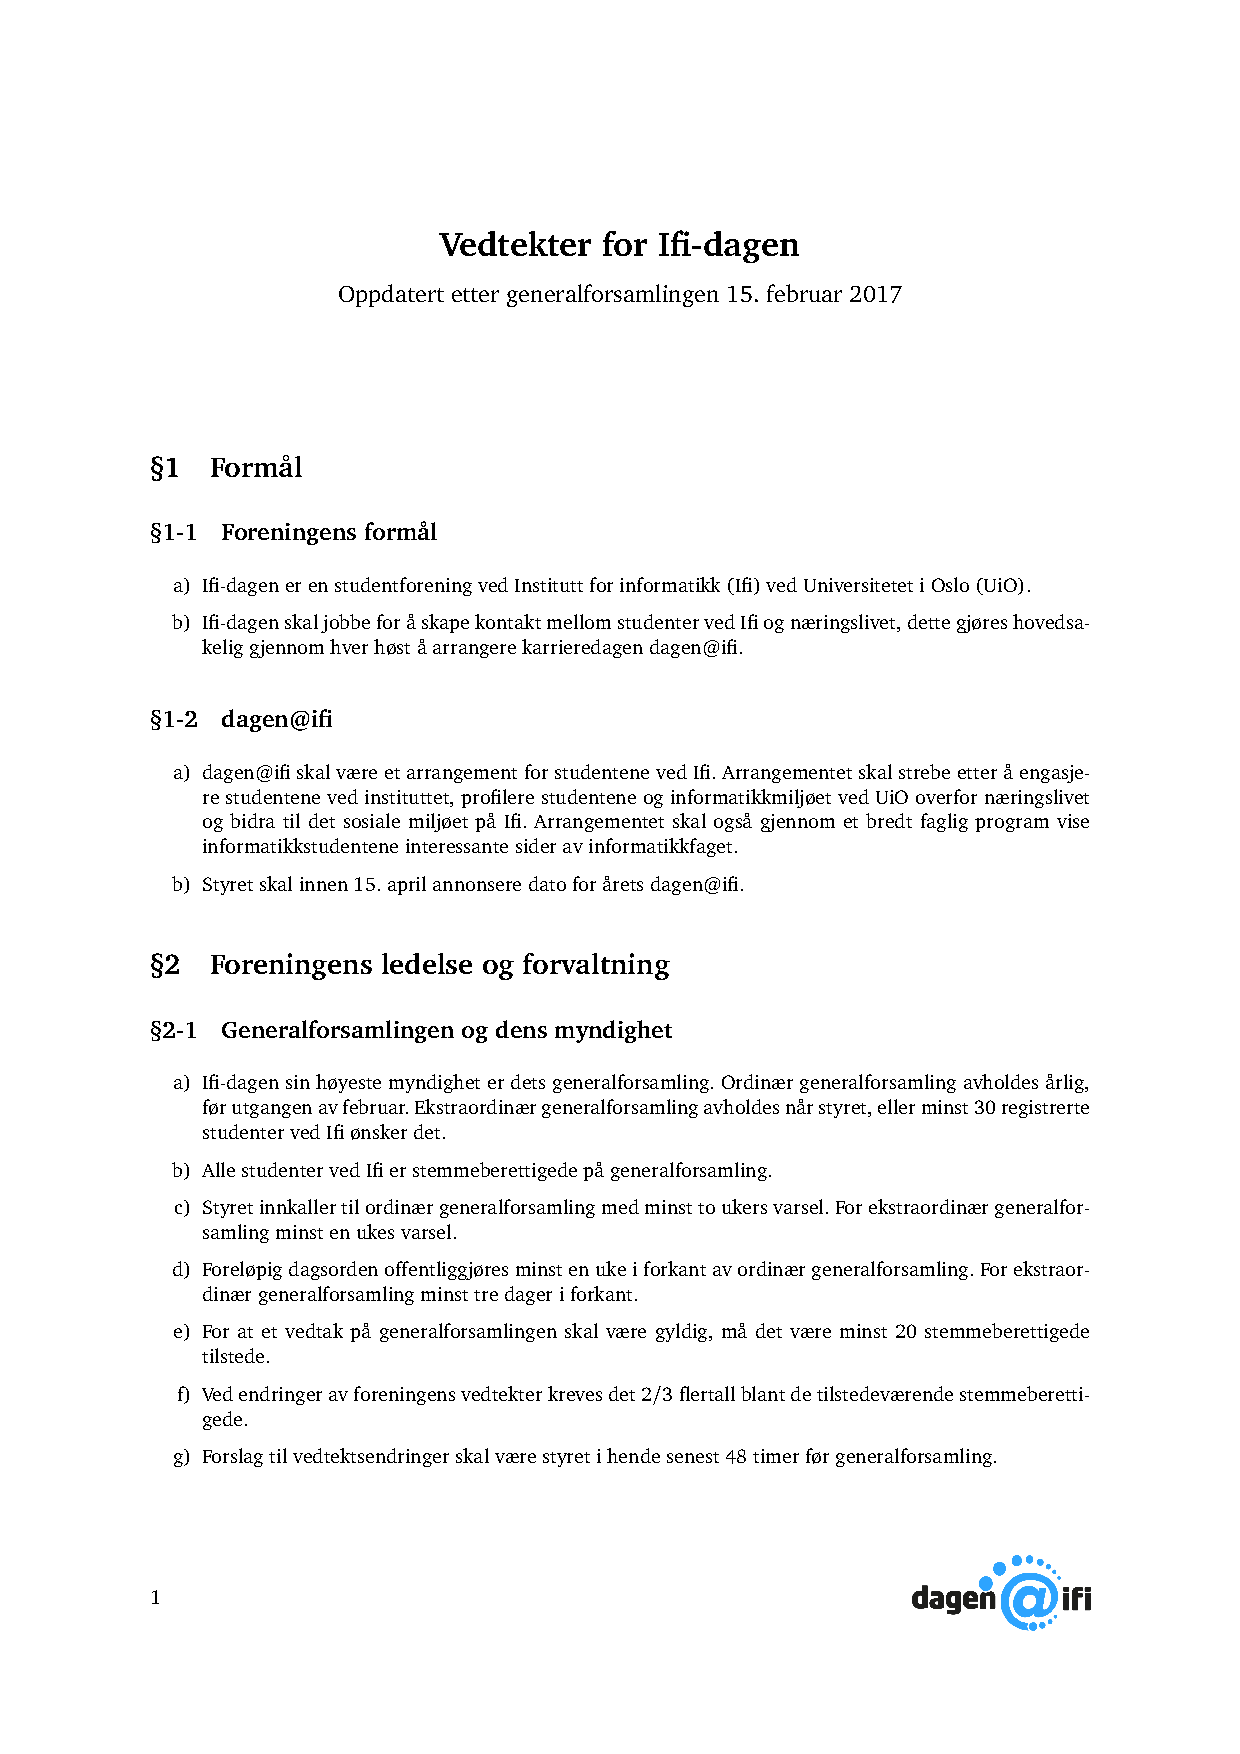
\includepdf[pages=-]{../../vedtekter/vedtekter.pdf}
\end{document}
